\documentclass[10pt,landscape]{article}
\usepackage{multicol,multirow}
\usepackage{calc}
\usepackage{ifthen}
\usepackage[landscape]{geometry}
\usepackage[colorlinks=true,citecolor=blue,linkcolor=blue]{hyperref}
\usepackage[fleqn]{amsmath}
\usepackage{amssymb,amsthm,amsfonts}
\usepackage{graphicx}
\usepackage{wrapfig}
\usepackage{cancel}
\usepackage{framed}
\usepackage[x11names]{xcolor}

\ifthenelse{\lengthtest { \paperwidth = 11in}}
{ \geometry{top=.3in,left=.3in,right=.3in,bottom=.3in} }
{\ifthenelse{ \lengthtest{ \paperwidth = 297mm}}
{\geometry{top=1cm,left=1cm,right=1cm,bottom=1cm} }
{\geometry{top=1cm,left=1cm,right=1cm,bottom=1cm} }
}
\pagestyle{empty}
\makeatletter
\renewcommand{\section}{\@startsection{section}{1}{0mm}%
{-1ex plus -.5ex minus -.2ex}%
{0.5ex plus .2ex}%x
{\normalfont\large\bfseries}}
\renewcommand{\subsection}{\@startsection{subsection}{2}{0mm}%
{-1explus -.5ex minus -.2ex}%
{0.5ex plus .2ex}%
{\normalfont\normalsize\bfseries}}
\renewcommand{\subsubsection}{\@startsection{subsubsection}{3}{0mm}%
{-1ex plus -.5ex minus -.2ex}%
{1ex plus .2ex}%
{\normalfont\small\bfseries}}
\renewcommand{\arraystretch}{1.3}
\makeatother
\setcounter{secnumdepth}{0}
\setlength{\parindent}{0pt}
\setlength{\parskip}{0pt plus 0.5ex}
\setlength{\mathindent}{0pt}
\setlength{\columnseprule}{0.2pt}

\definecolor{shadecolor}{RGB}{200,240,240}

\renewcommand{\CancelColor}{\color{purple}}
\newcommand{\utild}{\tilde{u}}

% -----------------------------------------------------------------------

\title{Partial Differential Equations}

\begin{document}
    \raggedright
    \footnotesize

    \begin{center}
        \textbf{Partial Differential Equations} \\
    \end{center}
    \begin{multicols}{3}
        \setlength{\premulticols}{1pt}
        \setlength{\postmulticols}{1pt}
        \setlength{\multicolsep}{1pt}
        \setlength{\columnsep}{2pt}

        \section{Domain and Boundary}
\begin{itemize}
    \item Domain $\Omega$ is an open subset of $\mathbb{R}^n$ (meaning all points are interior points)
    \item Boundary has to meet conditions:
    \item{ \emph{Dirichlet boundary conditions}: specify values $u$ on $\partial\Omega$: \\
        $u(x) = f(x)\ \forall x\in\partial\Omega$
    }
    \item{\emph{Neumann boundary conditions}: specify derivatives of $u$ on boundary.
    Only derivatives orthogonal to the boundary give additional information: \\
    normal derivative: $\frac{\partial u}{\partial n} = g(x)\ \forall x\in\partial\Omega$
    }
\end{itemize}

        \section{Classification}\label{sec:classification}
\begin{center}
    \makebox[\columnwidth]{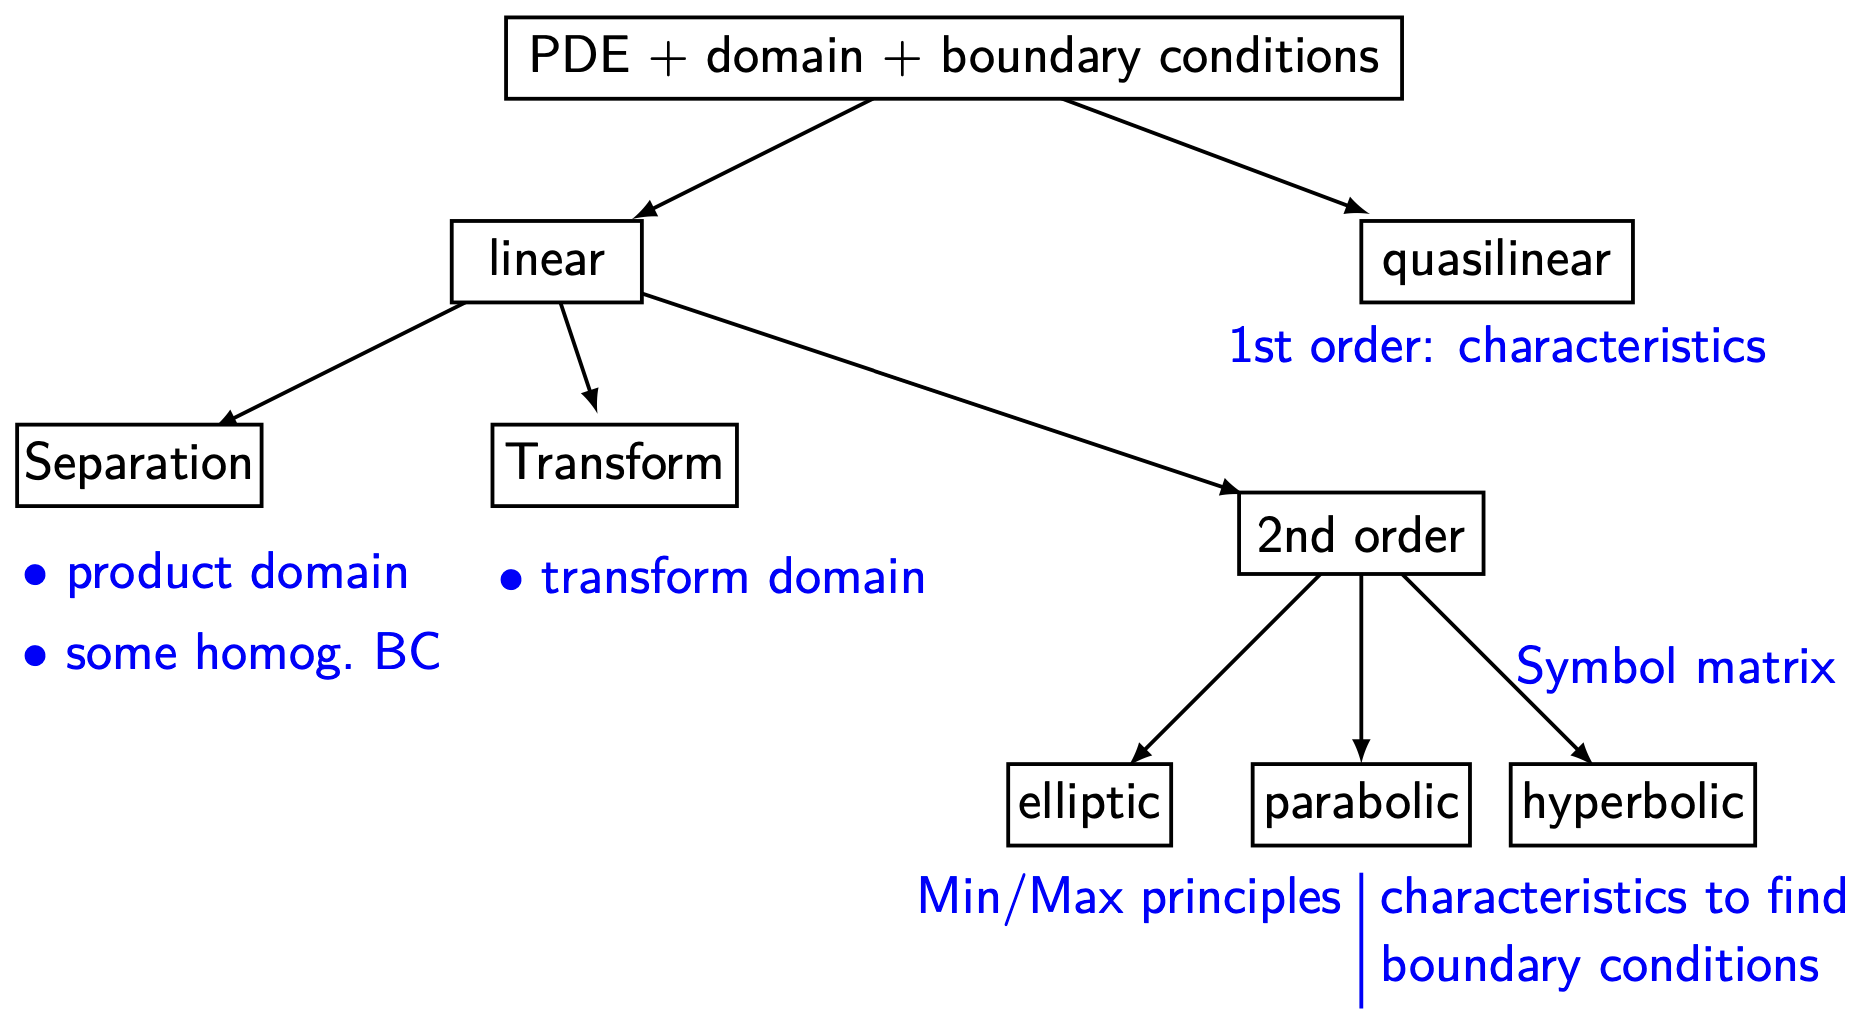
\includegraphics[width=0.9\columnwidth]{images/decision-tree}}
\end{center}

\subsection{Linearity}\label{subsec:linearity}
Given an equation involving a function $u(x), x\in\mathbb{R}$ and its derivatives,
there is a function $F$ describing the relation:
\begin{align*}
    F\left(
    \begin{matrix}
        x,y,z,p,q,s,t,r,\ldots                         \\
        \downarrow \text{(corresponding to)}\downarrow \\
        x, y, u, \frac{\partial u}{\partial x}, \frac{\partial u}{\partial y}, \frac{\partial^2 u}{\partial x^2},
        \frac{\partial^2 u}{\partial x\partial y},\frac{\partial^2 u}{\partial y^2}, \ldots
    \end{matrix}
    \right) = 0
\end{align*}
(common variable names $p_i\rightarrow\frac{\partial u}{\partial x_i}$ and
$t_{ij} \rightarrow\frac{\partial^2 u}{\partial x_i\partial x_j}$)

A PDE is \emph{linear} when function $F$ is linear in $u,p_1,\ldots,p_n,t_{11},\ldots,t_{nn},\ldots.$

A PDE is \emph{quasilinear} when function $F$ is linear in $p_1,\ldots,p_n,t_{11},\ldots,t_{nn},\ldots.$

For example, given the heat equation $u_t=\kappa u_{xx}$, $F$ would be $F(p_1,t_{22})=p_1-\kappa t_{22}$.

\symbolicsubsection{2\textsuperscript{nd} Order PDEs: Symbol Matrix}

The symbol matrix of the 2\textsuperscript{nd} order partial differential operator

\begin{align*}
    L=\sum_{i,j=1}^{n}a_{ij}(x)\frac{\partial^2}{\partial x_i \partial x_j}+\sum_{i=1}^n b_i(x)\frac{\partial}{\partial x_i}+c(x)
\end{align*}

is the symmetric matrix

\begin{align*}
    A=
    \begin{bmatrix}
        a_{11} & a_{12} & \ldots & a_{1n} \\
        a_{21} & a_{22} & \ldots & a_{2n} \\
        \vdots & \vdots & \ddots & \vdots \\
        a_{n1} & a_{n2} & \ldots & a_{nn}
    \end{bmatrix}
\end{align*}

For example:

\begin{center}
    \makebox[\columnwidth]{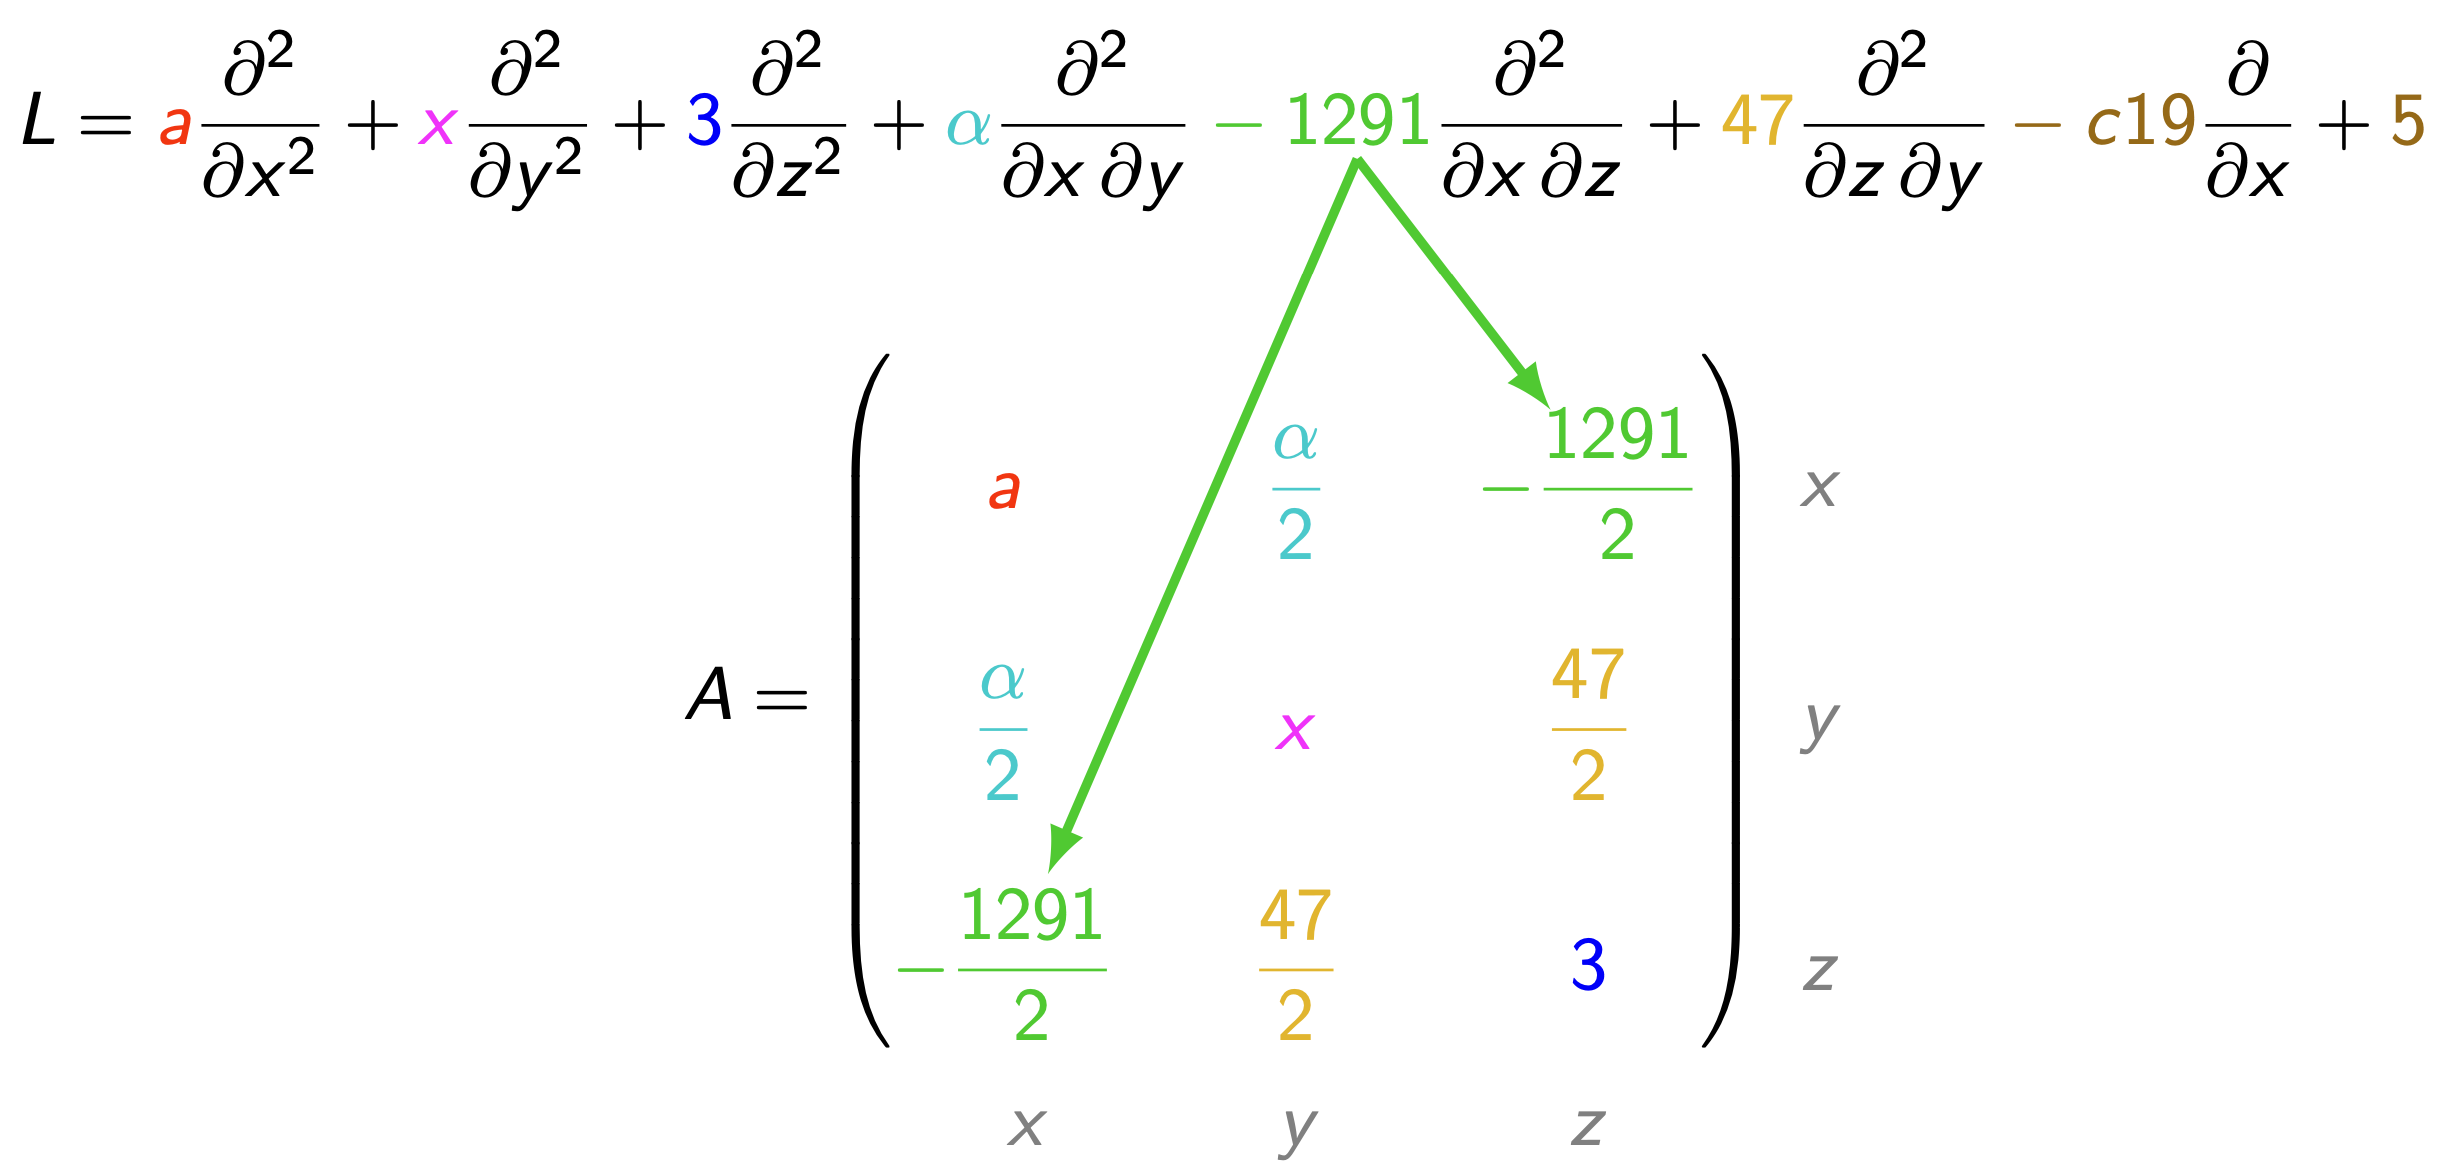
\includegraphics[width=0.9\columnwidth]{images/symbol-matrix}}
\end{center}

The type of equation can be inferred by the sign of the eigenvalues $\lambda_1,\ldots,\lambda_n$ of the symbol matrix.
Calculating the determinant ($\det A=\prod_i \lambda_i$) and trace ($\mathrm{tr}\ A=\sum_i \lambda_i$)
reveals information about the signs of its eigenvalues:

\subsubsection{Two Variables of PDE}

\begin{align*}
    \det A
    \left\{
    \begin{matrix}
        >0 & \text{elliptic (eigenvalues have same sign)}       \\
        =0 & \text{parabolic (at least one eigenvalue is zero)} \\
        <0 & \text{hyperbolic (eigenvalues have opposite sign)}
    \end{matrix}
    \right.
\end{align*}

\subsubsection{Three Variables of PDE}

\begin{align*}
    \mathrm{rank}\ A < 2 & \Rightarrow \text{not classified} \\
    \det A\text{ and }\mathrm{tr}\ A\text{ have different sign} & \Rightarrow\text{hyperbolic} \\
    \det A=0\text{, semidefinite (Cholesky decomp.)} & \Rightarrow\text{parabolic} \\
    A\text{ or }-A\text{ positive definite (Cholesky)} & \Rightarrow\text{elliptic} \\
    \text{all other cases} & \Rightarrow\text{hyperbolic}
\end{align*}

        \section{Quasilinear PDEs}\label{sec:quasilinear-pdes}

\subsection{Characteristics}\label{subsec:characteristics}

\begin{wrapfigure}{r}{0.4\columnwidth}
    \centering
    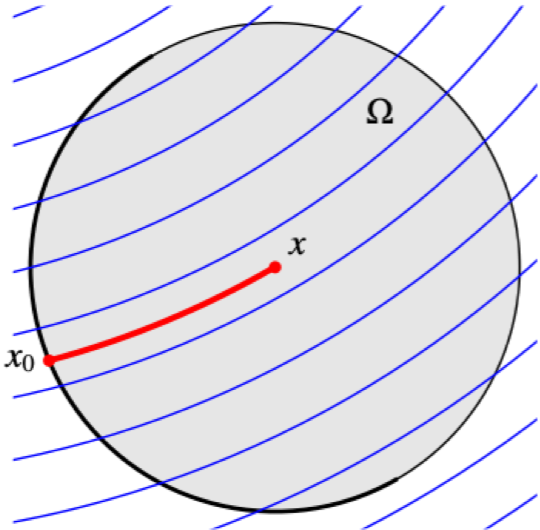
\includegraphics[width=0.4\columnwidth]{images/quasilinear}
\end{wrapfigure}

The PDE

\begin{align*}
    a(x,y,u)\frac{\partial u}{\partial x}+b(x,y,u)\frac{\partial u}{\partial y} = c(x,y,u)
\end{align*}

can be written in vector notation:

\begin{align*}
{\color{green}
\underbrace{
    \begin{pmatrix}
        a(x,y,u) \\
        b(x,y,u) \\
        c(x,y,u)
    \end{pmatrix}
}_{\vec t}
}
    \cdot
    {\color{black}
    \underbrace{
        \begin{pmatrix}
            \frac{\partial u}{\partial x} \\
            \frac{\partial u}{\partial y} \\
            -1
        \end{pmatrix}
    }_{\vec{n}}
    }
    &= 0
\end{align*}

where $\color{black}\vec{n}$ is a normal vector and $\color{green}\vec{t}$ is always tangential to the solution surface.
Therefore, we can elaborate a solution algorithm:
\begin{enumerate}
    \item{
        Using the Cauchy initial curve, we formulate
        \begin{align*}
            \vec{v}(s) = \begin{pmatrix}
                             v_x({\color{red}s} ) & v_y({\color{red}s}) & v_z({\color{red}s})
            \end{pmatrix}^T
        \end{align*}
        which is a point on the initial curve, parameterised by $s$.
    }
    \item{
        Find characteristic curves as solution of the ODEs

        \begin{align*}
            \frac{d}{d{\color{blue}t}}
            \begin{bmatrix}
                x({\color{blue}t}, {\color{red}s}) \\
                y({\color{blue}t}, {\color{red}s}) \\
                z({\color{blue}t}, {\color{red}s})
            \end{bmatrix}
            =
            \begin{bmatrix}
                a(x({\color{blue}t},{\color{red}s}), y({\color{blue}t},{\color{red}s}), z({\color{blue}t}, {\color{red}s})) \\
                b(x({\color{blue}t},{\color{red}s}), y({\color{blue}t},{\color{red}s}), z({\color{blue}t}, {\color{red}s})) \\
                c(x({\color{blue}t},{\color{red}s}), y({\color{blue}t},{\color{red}s}), z({\color{blue}t}, {\color{red}s}))
            \end{bmatrix}
        \end{align*}
        with
        \begin{align*}
            \begin{bmatrix}
                x({\color{blue}0}, {\color{red}s}) \\
                y({\color{blue}0}, {\color{red}s}) \\
                z({\color{blue}0}, {\color{red}s})
            \end{bmatrix}
            =
            \vec{v}({\color{red}s})
            =
            \begin{bmatrix}
                v_x({\color{red}s} ) \\
                v_y({\color{red}s})  \\
                v_z({\color{red}s})
            \end{bmatrix}
        \end{align*}
    }
    \item{
        Eliminate the variables {\color{blue}t} and {\color{red}s} and condense solution into a function $u(x, y)$:
        \begin{align*}
            \left.
            \begin{matrix}
                x=x({\color{blue}t},{\color{red}s}) \\
                y=y({\color{blue}t},{\color{red}s}) \\
                u=z({\color{blue}t},{\color{red}s})
            \end{matrix}
            \ \ \right\}
            \ u=u(x,y)
        \end{align*}
    }
\end{enumerate}

        \section{Linear PDEs}\label{sec:linear-pdes}
        \symbolicsubsection{Separation}\label{subsec:separation}
Conditions, when separation may be successful:

\begin{itemize}
    \item Homogeneous, linear PDE
    \item Homogeneous boundary conditions
    \item Domain must be a cartesian product (i.e. some form of rectangle when in cartesian coordinate system)
\end{itemize}

if these are given, we can try:

\begin{enumerate}
    \item Assume the structure of the solution to be in the form of some ansatz with separable variables, usually a product $u(x,y)=X(x)\cdot Y(y)$
    \item{
        Substitute $u$ in PDE with ansatz by variable:
        \begin{align*}
            \text{all terms of }x = \text{all terms of }y = {\color{red}\lambda}
        \end{align*}
        and solve the ordinary differential equations for $X(x)$ and $Y(y)$.
    }
    \item Use \emph{homogeneous} boundary conditions to determine admissible values ${\color{red}\lambda}_k$.
    \item Solve equations: $X_k(x)$ and $Y_k(y)$ $\Rightarrow u_k(x,y)=X_k(x)\cdot Y_k(y)$ using ansatz.
    \item Combine solutions: $u(x,y)=\sum_{k\in \mathbb{Z}}\left(a_ku_k(x,y)\right)$
    \item Use remaining boundary conditions to determine $a_k$.
\end{enumerate}

\paragraph{Separation Example}

Given the wave equation $\frac{\partial^2u}{\partial t^2}=\frac{\partial^2 u}{\partial x^2}$
for a string mounted between $u(0,t)=u(\pi,t)=0$ and is in the rest position at $t=0$: $u(x,0)=0$ but has initial velocity
$\frac{\partial u}{\partial t}(0,x)=\sin^3(x)=\frac{3}{4}\sin x-\frac{1}{4}\sin 3x$.
We choose the Ansatz $u(x,t)=X(x)T(t)$:

\begin{align*}
    \begin{matrix}
        X(x)T''(t)=X''(x)T(x) & |\div X(x)T(t) \\
        T''(t)\div T(t) = X''(x)\div X(x) = \mu
    \end{matrix} \\
\end{align*}
Hence, we receive the ODEs

\begin{align*}
    \mu T(t) = T''(t) \\
    \mu X(x) = X''(x)
\end{align*}
with $\mu < 0$ to receive oscillating solutions, the ODEs have the solutions

\begin{align*}
    X(x) & = C \sin(\sqrt\mu x)+\cancel{ D\cos(\sqrt\mu x) } \\
    T(t) & = A \sin(\sqrt\mu t)+B \cos(\sqrt\mu t)
\end{align*}
by taking into account the boundary conditions $X(0)=X(\pi)=0$, yielding $C=1,D=0$ and $\sqrt{n}\in\mathbb{N}$.
Therefore, we have the general solution
\begin{align*}
    u(x,t) & = \sum_{n=1}^\infty \sin(nx)\cdot\left( A_n\sin(nt)+B_n\cos(nt) \right) \\
    \ & = \sum_{n=1}^\infty A_n\sin(nx)\sin(nt) + \sum_{n=1}^\infty B_n\sin(nx)\cos(nt)
\end{align*}

considering the boundary conditions:
\begin{align*}
    u(x,0) = 0 = \sum_{n=1}^\infty B_n\sin(nx)\underbrace{\cos(0)}_{=1} \Rightarrow B_n=0
\end{align*}
and

\begin{align*}
    \ & \frac{\partial u}{\partial t} = \sum_{n=1}^\infty nA_n\sin(nx)\cos(nt)\\
    \ & \rightarrow \frac{\partial u}{\partial t}(x,0) = \sum_{n=1}^\infty nA_n\sin(nx) = \frac{3}{4}\sin x-\frac{1}{4}\sin 3x \\
    \ & \Rightarrow A_1=3/4, A_3=-1/12, A_{n\setminus \{1,3\}}=0 \\
    \ & \Rightarrow u(x,t)=(3/4)\sin(x)\sin(t)-(1/12)\sin(3x)\sin(3t)
\end{align*}

        \subsection{Transformation}\label{subsec:transformation}
\begin{enumerate}
    \item{
        Transform equation: derivatives turn into algebraic expressions:
        \begin{align*}
            \left(
            \mathcal{L}\frac{\partial u(t,y)}{\partial t}
            \right)(s) =
            s
            \underbrace{(\mathcal{L}f)(s, y)}_{=y_s(y)}
            -u(0,y)
        \end{align*}
    }
    \item{
        Transform y-boundary conditions: gives boundary conditions for
        \begin{align*}
            u(t,0) & =g(t) \\
            y_s(0)=(\mathcal{L}u(t,0))(s) & = (\mathcal{L}g)(s)
        \end{align*}
    }
    \item Solve PDE with fewer derivatives, ODEs
    \item Inverse transform
\end{enumerate}

\subsubsection{Laplace Transform}

(Only works on linear equations.)
The Laplace transform of a function $f:\mathbb{R}^+\to \mathbb{R}$ is the function

\begin{align*}
    \mathcal{L}f : \mathbb{R}^+\to \mathbb{R} : s \rightarrowtail \mathcal{L}f(s) = \int_0^\infty f(t)e^{-st}\ dt
\end{align*}

It is linear:

\begin{align*}
	\mathcal{L}(\alpha f+\beta f)=\alpha\mathcal{L}f+\beta\mathcal{L}f
\end{align*}

Example transformations:
\begin{align*}
	\begin{matrix}
		\text{Constant: } & \text{Exponential: } & \text{Derivative: } \\
		f(t)=c & f(t)=e^{-ct} & f(t)=g^{(n)}(t) \\
		(\mathcal{L}f)(s) = \frac{c}{s} & (\mathcal{L}f)(s) = \frac{1}{c+s} & (\mathcal{L}f^{(n)})(s)= \\
		& & -f^{(n-1)}(0)+s\left(\mathcal{L}f^{(n-1)}\right)(s) \\
		& & \text{(removes t-derivatives: }\frac{\partial}{\partial t}\rightarrow s\text{)}
	\end{matrix}
\end{align*}

\subsubsection{Fourier Transform}

For $f : \mathbb{R}\to\mathbb{C} : x \rightarrowtail f(x)$ the Fourier transform of $f$ is defined as

\begin{align*}
    \mathcal{F}f = \hat{f} : \mathbb{R}\to\mathbb{C} : k\rightarrowtail
    \frac{1}{\sqrt{2\pi}}\int_{-\infty}^{\infty}f(x)e^{-ikx}\ dx
\end{align*}

It turns the derivative $\frac{\partial}{\partial x}$ into a multiplication by $-ik$ (second derivatives are reduced to $i^2=-1$):
\begin{align*}
	(\mathcal{F}f^{(n)})(k) = (ik)^n\mathcal{F}f(k)
\end{align*}

The function $f$ can be recovered from $\hat{f}$ by
\begin{align*}
    f(x)=(\mathcal{F}^{-1}\hat{f})(x)
    = \frac{1}{\sqrt{2\pi}}\int_{-\infty}^\infty \hat{f}(k) e^{ikx}\ dk
\end{align*}

        \section{PDEs of Second Order}

Linear PDEs of second order have the form
\begin{align*}
	\sum_{i,j=1}^n a_{ij}\frac{\partial ^2}{\partial x_i\partial x_j}u+\sum_{i=1}^nb_i\frac{\partial}{\partial x_i}u + cu = f
\end{align*}

The equations fall into these categories:
\emph{Elliptic} (potential problem), \emph{parabolic} (heat equation, diffusion)
and \emph{hyperbolic} (wave equation, linearised supersonic flow).

\symbolicsubsection{Splitting the Solution}

Given a second order linear differential operator $L$,
we have the PDE $Lu = f \text{ in }\Omega$ with $u = g \text{ on }\partial\Omega$.

\begin{enumerate}
	\item We try to find a particular solution {\color{blue}$Lu_p = f$ in $\Omega$}, satisfying only the PDE and neglecting boundary conditions
	\item{
		To solve the original problem,
		we need an additional summand $u_r$ taking care of boundary values to receive the solution $u_p + u_r$.
		However, $u_r$ still needs to solve the PDE but due to linearity, this reduces to a homogeneous problem:
		\begin{align*}
			L(u_p + u_r) = f + Lu_r = f \Rightarrow{\color{blue} Lu_r = 0\text{ in }\Omega}
		\end{align*}
	}
	\item{
		Ensure that the boundary conditions are satisfied:
		\begin{align*}
			u_p+u_r = g \Rightarrow {\color{blue}u_r = g - u_p\text{ on }\partial\Omega}
		\end{align*}
	}
	\item{
		If the solution is not unique, we're able to find other solutions using an additional term $u_h$:
		\begin{align*}
			L(u_p + u_r + u_h) = f + Lu_h &\ \Rightarrow Lu_h = 0\text{ in }\Omega \\
			u_p + u_r + u_h = g + u_h &\ \Rightarrow u_h = 0\text{ on }\partial\Omega
		\end{align*}
	}
\end{enumerate}

For example, consider the PDE $\nabla^2 u = 4$ in $\Omega = \{(x,y)\ |\ x^2 + y^2 < 1\}$ and $u = 0.5x+0.5$ on $\partial\Omega$.
This has the particular solution $u_p(x,y)=x^2+y^2$.
To fix boundary conditions, we find a solution $u_r$ of the homogeneous problem with boundary values
$u_r = 0.5x + 0.5 - u_p(x,y) = 0.5x + 0.5 - \underbrace{1}_{\text{on }\partial\Omega} = 0.5x - 0.5$ giving the complete solution
$u(x,y) = u_p(x,y) + u_r(x,y) = x^2 + y^2 + 0.5x - 0.5$.

        \section{Elliptic PDEs}
\subsection{Maximum Principle for Elliptic Operators}
Theorem: If $L$ is an elliptic differential operator on a connected and bounded domain $\Omega$,
and $u$ is a solution $Lu = 0$, then $u$ takes its maximum and minimum on the boundary of $\Omega$.

\subsection{Uniqueness of Solutions}
Theorem: If $L$ is an elliptic differential operator on a connected and bounded domain $\Omega$,
then there is at most one solution of $Lu = f$ with boundary conditions $u_{|\partial\Omega} = g$.

        \section{Numerical Methods}
\subsection{Discretisation of Operators}

\begin{align*}
	\frac{\partial g}{\partial x}
	\approx
	\frac{g(x + \Delta x) - g(x)}{\Delta x}
\end{align*}

\begin{align*}
	\frac{\partial^2 g}{\partial x^2}
	\approx
	\frac{g(x + \Delta x) - 2\cdot g(x) + g(x - \Delta x)}{\Delta x^2}
\end{align*}

($\Delta$ referring to step size)
\subsection{Finite Elements}

We have a set of given local basis functions $v_1(x), \ldots, v_n(x)$ that are continuous and piecewise differentiable.
We subdivide $\Omega$ into meshes and assign each nodal point a nodal variable $a_k$.
Then, we use shape functions to represent the PDE on the mesh,
e.g. using triangular functions $l_1(x)=1-x$ and $l_2(x) = x$ to obtain \emph{local} element matrices
\begin{align*}
	E = 
	\begin{bmatrix}
		\int_0^1 l_1^\prime(s)\cdot l_1^\prime(s)\ ds & \int_0^1 l_1^\prime(s)\cdot l_2^\prime(s)\ ds \\
		\int_0^1 l_2^\prime(s)\cdot l_1^\prime(s)\ ds & \int_0^1 l_2^\prime(s)\cdot l_2^\prime(s)\ ds
	\end{bmatrix}
	=
	\begin{bmatrix}
		1 & -1 \\
		-1 & 1
	\end{bmatrix}
\end{align*}

that can then be used to construct the mesh matrix $M=1/h\cdot E$ using mesh size $h$.
Afterwards, the global Ritz matrix can be computed, e.g. for a one-dimensional mesh with 4 nodal points and 2 unknown inner points,
yielding 4 base functions $v_1,v_2,v_3,v_4$:

\begin{align*}
	R^4 = \begin{bmatrix}
		{\color{red} M^{(1)}_{0,0}} & \color{red}{M^{(1)}_{0,1}} & 0 & 0 \\
		{\color{red} M^{(1)}_{1,0}} & {\color{red} M^{(1)}_{1,1}} + {\color{blue} M^{(2)}_{0,0}} & {\color{blue} M^{(2)}_{0,1}} & 0 \\
		0 & {\color{blue} M^{(2)}_{1,0}} & {\color{blue} M^{(2)}_{1,1}} + {\color{green} M^{(3)}_{0,0}} & {\color{green} M^{(3)}_{0,1}} \\
		0 & 0 & {\color{green} M^{(3)}_{1,0}} & {\color{green} M^{(3)}_{1,1}}
	\end{bmatrix}
\end{align*}

The system vector can then be calculated:

\begin{align*}
	\vec{r^4} = \begin{pmatrix}
		\int_0^1 f(x)\cdot v_0(x)\ dx \\
		\vdots \\
		\int_0^1 f(x)\cdot v_3(x)\ dx
	\end{pmatrix}
\end{align*}

Finally, we have obtained the Ritz system: $R^4\cdot\vec{a}=\vec{r^4}$.
That yields the approximation function (as defined by the ansatz): $\tilde{u}(x)=\sum_{i=0}^3 a_i\cdot v_i(x)$
3with $a_0$ and $a_3$ fulfilling the boundary conditions.
        \section{Finite Difference Method for Elliptic PDEs}

In case of a one-dimensional domain:
\begin{enumerate}
	\item Given the differential equation $Lu(x) = f(x)$
	\item{
		Discretise domain.
		E.g. we have $x_k^{(n)}=k\cdot\Delta x$ with $\Delta x = 1 / n$.
	}
	\item Discretise equation using discrete operators
	\item{
		Replace functions $u(x)$ and $f(x)$ by vectors of nodal values:
		$u_k^{(n)}=u\left(x_k^{(n)}\right)$ and $f_k^{(n)} = f\left(x_k^{(n)}\right)$
	}
	\item Solve for $A^{(n)}\cdot \tilde{u}^{(n)} = f^{(n)}$ for inner knots while considering boundary conditions.
\end{enumerate}

\subsection{One-Dimensional Example}

The boundary value problem $u''(x) = 4\cdot(u(x) - x)=4u(x)-4x,\quad x\in ]0,1[$ with $u(0) = 0$ and $u(1) = 2$
should be approximated by function $\tilde{u}(x)$ using FDM with $\Delta x = 1/4$.

The discretised equation therefore is:
\begin{align*}
	\frac{u_{k+1} - 2u_k + u_{k-1}}{\Delta x^2} = 4u_k - 4x_k\quad(k=1,\ldots,n-1)
\end{align*}

\makebox[\columnwidth]{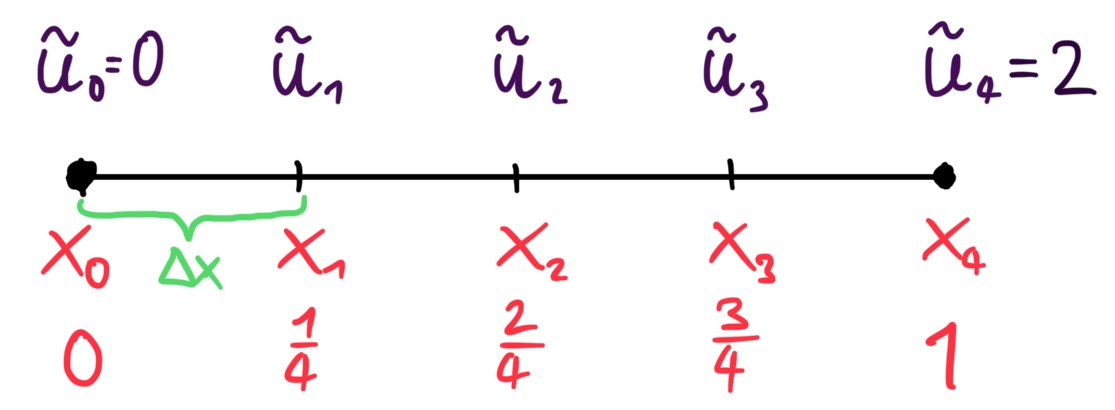
\includegraphics[width=0.6\columnwidth]{images/FDM_Elliptic}}

giving us the linear system
\begingroup
\renewcommand*{\arraystretch}{3}
  \begin{align*}
    \left|
    \begin{matrix}
      \frac{\tilde{u}_2 - 2\tilde{u}_1 + \cancelto{=0}{\tilde{u}_0}}{\cancelto{= 1/16}{\Delta x^2}} & = 4\tilde{u}_1 - 4\cancelto{1/4}{x_1} \\
      \frac{\tilde{u}_3 - 2\tilde{u}_2 + \tilde{u}_1}{\cancelto{= 1/16}{\Delta x^2}} & = 4\tilde{u}_2 - 4\cancelto{2/4}{x_2} \\
      \frac{\cancelto{= 2}{\tilde{u}_4} - 2\tilde{u}_3 + \tilde{u}_2}{\cancelto{= 1/16}{\Delta x^2}} & = 4\tilde{u}_3 - 4\cancelto{3/4}{x_3} \\
    \end{matrix}
    \right|
  \end{align*}
\endgroup

resulting in
\begin{align*}
	-32\utild_1 + 16\utild_2 & = 4\utild_1 - 1\quad\rightarrow -36\utild_1 + 16\utild_2 = -1 \\
	16\utild_1 - 32\utild_2 + 16\utild_3 & = 4\utild_2 - 2\quad\rightarrow 16\utild_1 - 36\utild_2 + 16\utild_3 = -2 \\
	16\utild_2 - 32\utild_3 + 16\cdot 2 & = 4\utild_3 - 3\quad\rightarrow 16\utild_2 - 36\utild_3 = -35
\end{align*}

ultimately giving the equation in matrix form (optional):
\begin{align*}
	\begin{bmatrix}
		-36 & 16 & 0 \\
		16 & -36 & 16 \\
		0 & 16 & -36
	\end{bmatrix}
	\cdot
	\begin{bmatrix}
		\utild_1 \\
		\utild_2 \\
		\utild_3 \\
	\end{bmatrix}
	=
	\begin{bmatrix}
		-1 \\
		-2 \\
		-35
	\end{bmatrix}
\end{align*}

giving the approximation vector $\utild \approx (0.4, 0.83, 1.34)$.

\subsection{Two-Dimensions Example}

We have Poisson's differential equation $-\Delta u(x,y)=f(x,y)$ with
$f(x,y) = \left( (3x+x^2)\cdot y(1-y) + (3y+y^2)\cdot x(1-x) \right)\cdot e^{x+y}$ on
$\Omega = [0,1]\times [0,1]$ with homogeneous boundary conditions.
Setting $h=\Delta x = \Delta y = \frac{1}{3}$, we can use the discrete Laplace operator.
Discretisation of the geometry yields
\makebox[\columnwidth]{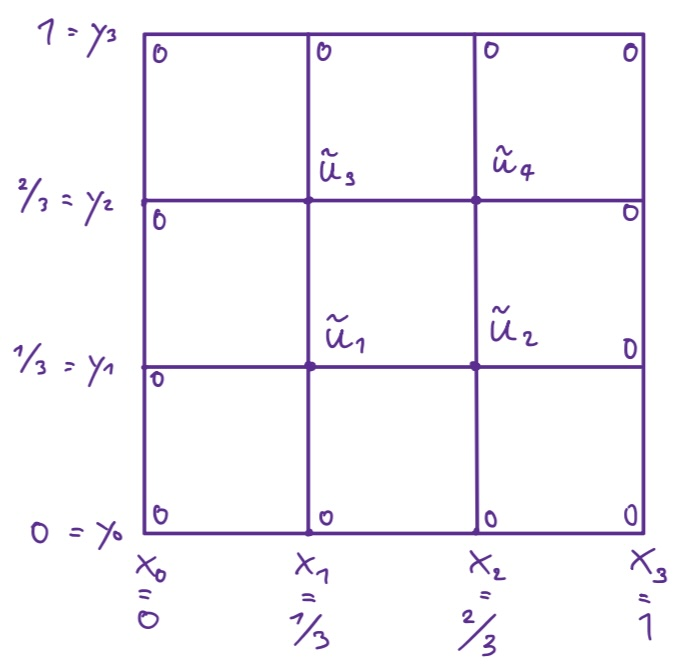
\includegraphics[width=0.5\columnwidth]{images/fdm_elliptic_2d}}

and we can define for each inner node an equation:
\begin{align*}
	u_1 & : -\frac{\utild_2 + \utild_3 + \cancelto{0}{y_1} + \cancelto{0}{x_1} - 4\utild_1}{\cancelto{(1/3)^2}{1/h^2}} = f(1/3, 1/3) = f_1 \\
	u_2 & : -\frac{0 + \utild_4 + \utild_1 + 0 - 4\utild_2}{(1/3)^2} = f(2/3, 1/3) = f_2 \\
	u_3 & : -\frac{\utild_4 + 0 + 0 + \utild_1 - 4\utild_3}{(1/3)^2} = f(1/3, 2/3) = f_3 \\
	u_4 & : -\frac{0 + 0 + \utild_3 + \utild_2 - 4\utild_4}{(1/3)^2} = f(2/3, 2/3) = f_4 \\
\end{align*}

giving the linear system:
\begin{align*}
	-9\cdot\begin{bmatrix}
		{\color{blue}-4} & {\color{blue}1} & {\color{purple}1} & {\color{purple}0} \\
		{\color{blue}1} & {\color{blue}-4} & {\color{purple}0} & {\color{purple}1} \\
		{\color{purple}1} & {\color{purple}0} & {\color{blue}-4} & {\color{blue}1} \\
		{\color{purple}0} & {\color{purple}1} & {\color{blue}1} & {\color{blue}-4}
	\end{bmatrix}
	\begin{bmatrix}
		\utild_1 \\
		\utild_2 \\
		\utild_3 \\
		\utild_4
	\end{bmatrix}
	=
	\begin{bmatrix}
		f_1 \\
		f_2 \\
		f_3 \\
		f_4
	\end{bmatrix}
\end{align*}

        \section{Finite Differences Method for Parabolic PDEs}

\numericsubsection{Richardson's \em{Explicit} FD Scheme}

\begin{enumerate}
	\item \emph{Discretise parabolic PDE} $Lu(...) = f(...)$ using discrete operators
	\item{
		\emph{Discretise geometry} by introducing a grid:
		$x_{j,k} = (j\cdot\Delta x, k\cdot\Delta t)$ with $j$ as the local index
		and $k$ as the time index where $k=0$ is on boundary
		and \colorbox{shadecolor}{$\Delta x = \frac{1}{n}$},
		\colorbox{shadecolor}{$\Delta t = \frac{r}{n^2}$}
		and \colorbox{shadecolor}{$r = \frac{\Delta t}{\Delta x^2}$}
	}
	\item{
		\emph{Introduce approximated nodal values} $\utild(x_{j,k}) = \utild_{j,k}$ and $f_j = f(x_j,0)$ for the Dirichlet boundary conditions.
	}
	\item{
		Find a matrix $C$ that satisfies

		\colorbox{shadecolor}{$
			\displaystyle
			\utild_{j}^{(k+1)}=r\utild_{j-1}^{(k)}+(1-2r)\utild_{j}^{(k)} + r\cdot \utild_{j+1}^{(k)}
		$}

		for inner grid points for each ``step`` satisfying boundary conditions: $\utild_{j}^{(0)}=\utild_{j,0}=f_j$
	}
	\item{
		Iteratively generate solution vector using $\utild^{(k+1)}=C\cdot\utild^{(k)}$
		(i.e. $\utild^{(k)} = C^k\cdot \vec{f}$)
	}
\end{enumerate}

\subsubsection{Stability Analysis}

\begin{wrapfigure}{r}{0.25\columnwidth}
	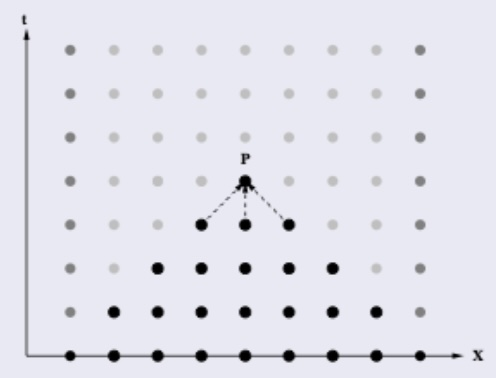
\includegraphics[width=0.25\columnwidth]{images/richardsons}
\end{wrapfigure}

The scheme of Richardson tends asymptotically to zero with k to infinity if
for eigenvalues of $C$, $|\lambda_\mathrm{max}|<1$ is true or $||C^{(n)}||<1$ with respect to the spectral norm of C.

We only receive a good approximation if the steps are small enough to ``catch'' enough information on the boundary.

\subsubsection{Example Using Heat Equation}

\textbf{Given} the heat equation $\frac{\partial u}{\partial t}(x,t) = \frac{\partial^2 u}{\partial x^2}(x,t)$
for the domain $\Omega = [0,1]\times [0, \infty[$ with the boundary conditions
$u(x,0) = e^x$, $u(0,t) = e^t$ and $u(1,t) = e^{1+t}$, we want to find an approximation $\utild$ for points
$(\sfrac{1}{3},\sfrac{2}{3}),(\sfrac{2}{3},\sfrac{2}{3})$ using $\Delta x = \sfrac{1}{3}$ and $\Delta t = \sfrac{1}{3}$.

\textbf{Discretisation of Heat Equation}:
\begin{align*}
	& \frac{u(x,t+\Delta t)-{\color{blue} u(x,t)}}{\color{blue}\Delta t}\approx\frac{u(x+\Delta x,t)-2\cdot u(x,t)+u(x-\Delta x,t)}{\Delta x^{2}} \\
	& u(x,t+\Delta t)\approx {\color{blue}u(x,t)+\Delta t}\cdot{\frac{u(x+\Delta x,t)-2 u(x,t)+u(x-\Delta x,t)}{\Delta x^{2}}} \\
	& \utild_{j,k+1}=u_{j,k}+r\cdot u_{j+1,k} - 2u_{j,k} + u_{j-1,k}\quad {\color{gray}\left|\ r=\frac{\Delta t}{\Delta x^2}\right.} \\
	& \utild_{j,k+1} = r\cdot\utild_{j-1,k}+(1-2r)\utild_{j,k} + r\cdot\utild_{j+1,k}
\end{align*}

\textbf{Discretisation of Geometry}:

\makebox[\columnwidth]{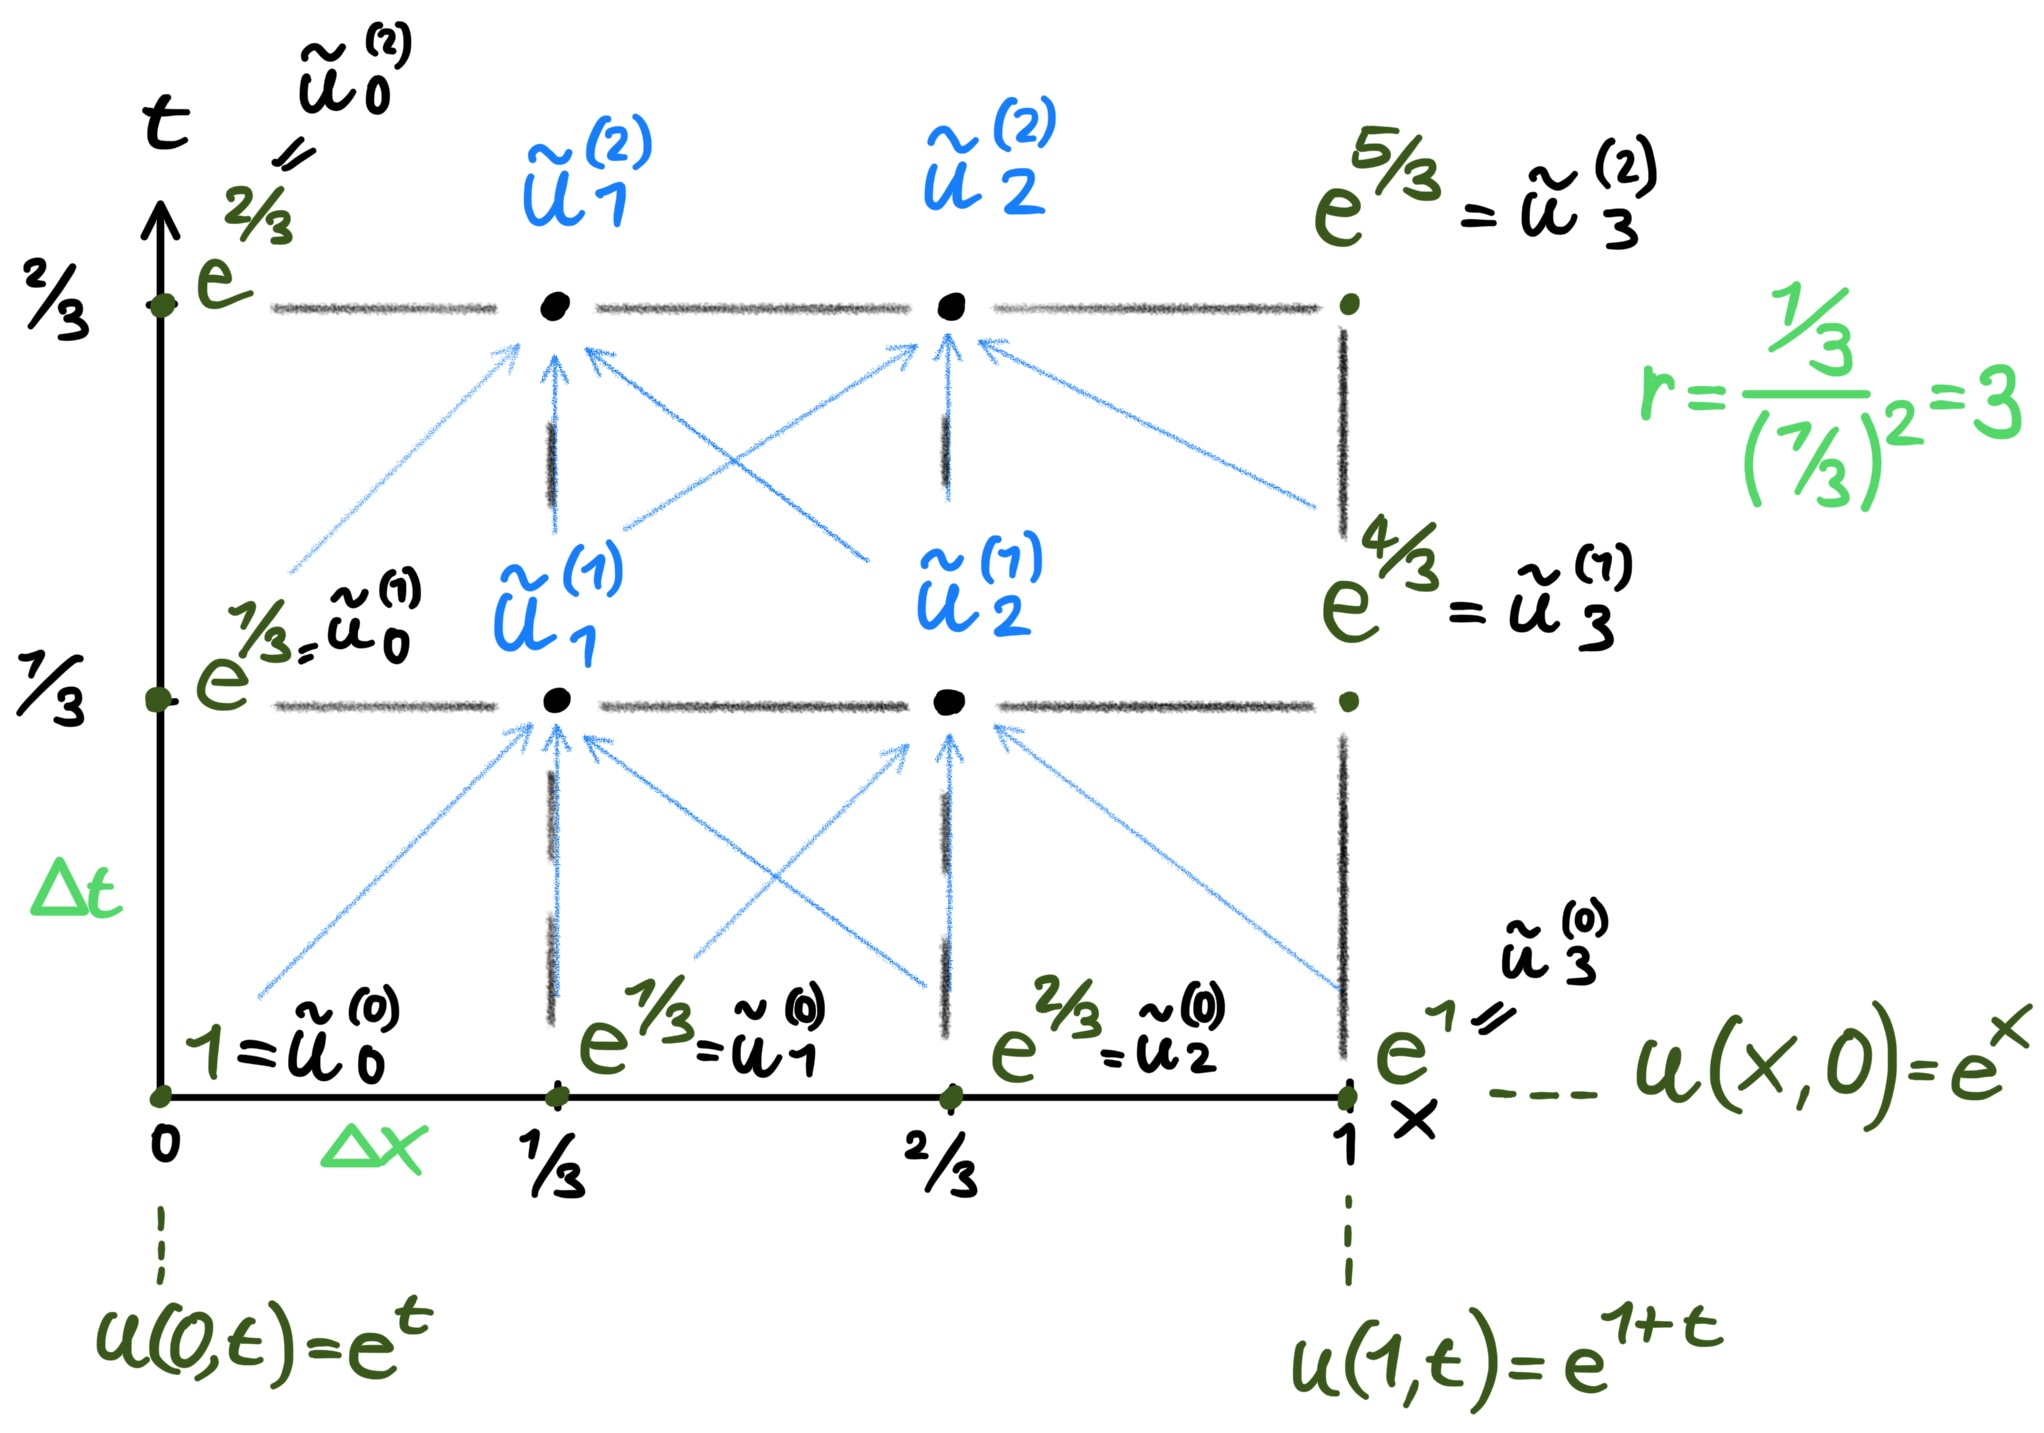
\includegraphics[width=0.75\columnwidth]{images/richardson_explicit}}

\textbf{Solution Method:} With $r$ having a set value, we can write the iterative equation as:
\begin{align*}
	\utild_{j}^{(k+1)} = 3\utild_{j-1}^{(k)} + 5\utild_{j}^{(k)} + 3\utild_{j+1}^{(k)}
\end{align*}

and thus, for $\mathbf{k+1=1}$:
\begin{align*}
	\utild_1^{(1)} & = 3\cancelto{1}{\utild_0^{(0)}} - 5\cancelto{e^{\sfrac{1}{3}}}{\utild_1^{(0)}} + 3\cancelto{e^{\sfrac{2}{3}}}{\utild_2^{(0)}} {\color{gray} = 1.8651} \\
	\utild_2^{(1)} & = 3\utild_1^{(0)} - 5\utild_2^{(0)} + 3\utild_3^{(0)} {\color{gray} = 2.603}
\end{align*}

and $\mathbf{k+1 = 2}$:
\begin{align*}
	\utild_1^{(2)} & = 3\cancelto{e^{\Delta t\cdot k}}{\utild_0^{(1)}} - 5\utild_1^{(1)} + 3\utild_2^{(1)} {\color{gray} = 2.6702} \\
	\utild_2^{(2)} & = 3\utild_1^{(1)} - 5\utild_2^{(1)} + 3\cancelto{e^{1+\Delta t\cdot k}}{\utild_3^{(1)}} {\color{gray} = 3.9614}
\end{align*}

Alternatively, using matrix $C$:
\begin{align*}
	\begin{bmatrix}
		\utild_1 \\
		\utild_2
	\end{bmatrix}^{(k+1)}
	=
	\underbrace{
		\begin{bmatrix}
			-5 & 3 \\
			3 & -5
		\end{bmatrix}
	}_{C}
	\begin{bmatrix}
		\utild_1 \\
		\utild_2
	\end{bmatrix}^{(k)}
	+
	\underbrace{
		3\begin{bmatrix}
			e^{\Delta t k} = e^\frac{k}{3} \\
			e^{1+\Delta t k} = e^{1+\frac{k}{3}}
		\end{bmatrix}
	}_\text{Dirichlet B.C.}
\end{align*}

and
\begin{align*}
	\begin{bmatrix}
		\utild_1 \\
		\utild_2
	\end{bmatrix}^{(2)}
	=
	C^2\vec{\utild}^{(0)} + C\cdot 3\begin{bmatrix}
		1 \\
		e
	\end{bmatrix}
	+
	3\begin{bmatrix}
		e^{\sfrac{1}{3}} \\
		e^{\sfrac{4}{3}}
	\end{bmatrix}
	{\color{gray}
		=
		\begin{bmatrix}
			2.6702 \\
			3.9614
		\end{bmatrix}
	}
\end{align*}

\numericsubsection{Richardson's \em{Implicit} Scheme}

Uses a backward finite difference for the discretisation in $t$:
\begin{align*}
	\frac{\partial u}{\partial t} \approx \frac{u(x,t) - u(x, t-\Delta t)}{\Delta t}
\end{align*}
to be able to consider all boundary points.
We therefore look for a matrix $E$ to receive a system of linear equations:
\begin{align*}
	E\cdot \utild^{(k+1)} = \utild^{(k)}
\end{align*}
and get a solution by inverting (of course not suitable for numerical tasks, only theoretical):
\begin{align*}
	\utild^{(k+1)} = \left(E^{(n)}\right)^{-1}\cdot\utild^{(k)}
\end{align*}

The method is stable independently of $r$ (absolute stability).

\subsubsection{Example}

\textbf{Given} the heat equation $\frac{\partial u}{\partial t}(x,t) = \frac{\partial^2 u}{\partial x^2}(x,t)$
for the domain $\Omega = [0,2]\times [0, \infty[$ with boundary condition
$u(x,0) = \sin\left(\frac{\pi x}{2}\right)$. We want to find $\utild(x,0.1)$ using $\Delta x = 0.5$ and $\Delta t = 0.05$.
\\[1em]
\textbf{Discretisation of Heat Equation}
analogously like in the explicit method:
\begin{align*}
	\tilde{u}_{j}^{(k)}=-r\cdot\utild_{j-1}^{(k+1)}+(1+2\cdot r)\cdot\tilde{u}_{j}^{(k+1)}-r\cdot\tilde{u}_{j+1}^{(k+1)}
\end{align*}

\textbf{Discretisation of Geometry}

\makebox[\columnwidth]{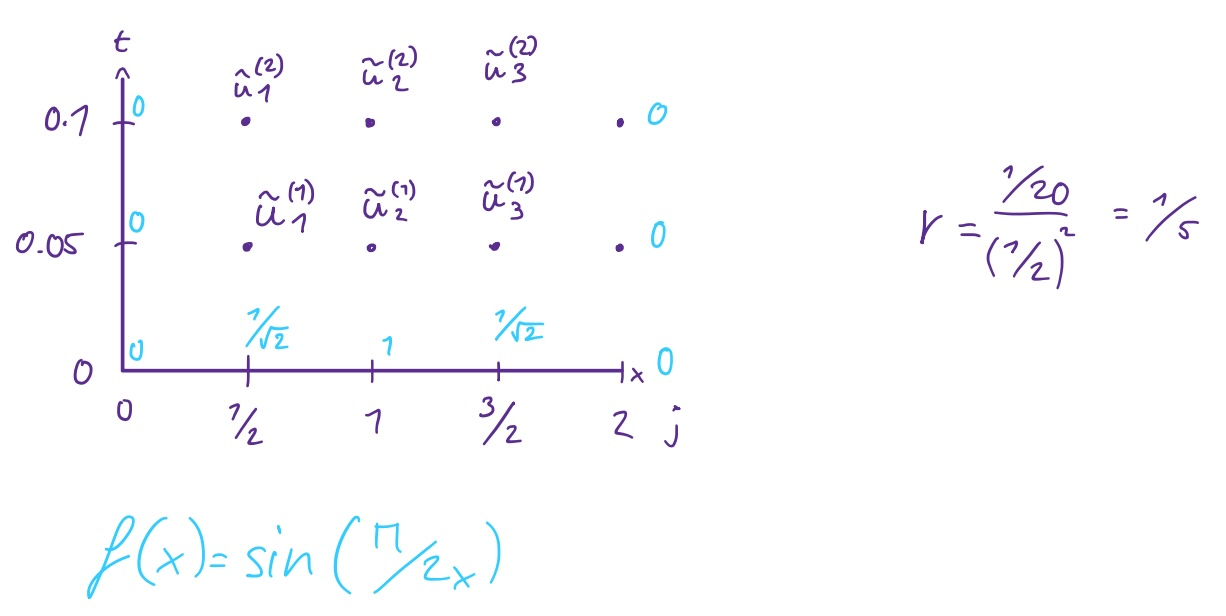
\includegraphics[width=\columnwidth]{images/richardson_implicit}}

\textbf{Solution}

For $k=0$:
\begin{align*}
	\mathbf{j=1} : & -\cancelto{\frac{1}{5}}{r}\cdot\cancelto{\color{cyan}0}{\utild_{0}^{(1)}} + \sfrac{7}{5}\cdot\utild_1^{(1)} - \cancelto{\frac{1}{5}}{r}\cdot\utild_2^{(1)} = f(\sfrac{1}{2}) = {\color{cyan}\sfrac{1}{\sqrt{2}}} \\
	\mathbf{j=2} : & -\cancelto{\frac{1}{5}}{r}\cdot\utild_{1}^{(1)} + \sfrac{7}{5}\cdot\utild_2^{(1)} - \cancelto{\frac{1}{5}}{r}\cdot\utild_3^{(1)} = f(1) = {\color{cyan}1} \\
	\mathbf{j=3} : & -\cancelto{\frac{1}{5}}{r}\cdot\utild_{2}^{(1)} + \sfrac{7}{5}\cdot\utild_3^{(1)} - \cancelto{\frac{1}{5}}{r}\cdot\cancelto{\color{cyan}0}{\utild_4^{(1)}} = f(\sfrac{3}{2}) = {\color{cyan}\sfrac{1}{\sqrt{2}}} \\
\end{align*}

resulting in the linear system
\begin{align*}
	\underbrace{
		\begin{bmatrix}
			\sfrac{7}{5} & -\sfrac{1}{5} & 0 \\
			-\sfrac{1}{5} & \sfrac{7}{5} & -\sfrac{1}{5} \\
			0 & -\sfrac{1}{5} & \sfrac{7}{5}
		\end{bmatrix}
	}_{E}
	\begin{bmatrix}
		\utild_1 \\
		\utild_2 \\
		\utild_3 \\
	\end{bmatrix}^{(1)}
	=
	\begin{bmatrix}
		\sfrac{1}{\sqrt{2}} \\
		1 \\
		\sfrac{1}{\sqrt{2}}
	\end{bmatrix}
	& \Rightarrow
	\begin{bmatrix}
		\utild_1 \\
		\utild_2 \\
		\utild_3 \\
	\end{bmatrix}^{(1)}
	\approxeq
	{\color{purple}
	\begin{bmatrix}
		0.633 \\
		0.895 \\
		0.633
	\end{bmatrix}
	} \\
	\overbrace{
		\begin{bmatrix}
			\sfrac{7}{5} & -\sfrac{1}{5} & 0 \\
			-\sfrac{1}{5} & \sfrac{7}{5} & -\sfrac{1}{5} \\
			0 & -\sfrac{1}{5} & \sfrac{7}{5}
		\end{bmatrix}
	}
	\begin{bmatrix}
		\utild_1 \\
		\utild_2 \\
		\utild_3 \\
	\end{bmatrix}^{(2)}
	= {\color{purple}
	\begin{bmatrix}
		0.633 \\
		0.895 \\
		0.633
	\end{bmatrix}
	}
	& \Rightarrow
	\begin{bmatrix}
		\utild_1 \\
		\utild_2 \\
		\utild_3 \\
	\end{bmatrix}^{(2)}
	\approxeq
	\begin{bmatrix}
		0.567 \\
		0.801 \\
		0.567
	\end{bmatrix}
\end{align*}

\numericsubsection{Crank-Nicolson Scheme}

Averaging the explicit and implicit method of Richardson to improve error term:
\begin{align*}
	g^{\prime}(x)={\frac{1}{2}}\cdot\left({\frac{g(x+\Delta x)-g(x)}{\Delta x}}+{\frac{g(x)-g(x-\Delta x)}{\Delta x}}\right)
	+ \mathcal{O}(\Delta x^{2})
\end{align*}

The Crank-Nicolson values at time-level $k+1$ are computed by solving the system of linear equations
\begin{align*}
	F^{(n)}\cdot\vec{\utild}^{(k+1)} = G^{(n)}\cdot\vec{\utild}^{(k)}
\end{align*}

which can formally be transformed into the linear iteration
\begin{align*}
	\vec{\utild}^{(k+1)}=\left(F^{(n)}\right)^{-1}\cdot G^{(n)}\cdot\vec{\utild}^{(k)}
\end{align*}

where the matrices $F$ and $G$ are for the heat equation $u_t=u_{xx}$:
\begin{align*}
	& F^{(n)}=E^{(n)}+I=\mathrm{tridiag}_{n-1}(-r,2+2\cdot r,-r) \\
	& G^{(n)}=C^{(n)}+I=\mathrm{tridiag}_{n-1}(r,2-2\cdot r,r)
\end{align*}

with
\begin{align*}
	E^{(n)}=\mathrm{tridiag}_{n-1}(-r,1+2\cdot r,-r)	\quad\text{(from implicit)}
\end{align*}
and
\begin{align*}
	C^{(n)}=\mathrm{tridiag}_{n-1}(r,1-2\cdot r,r)\quad\text{(from explicit)}
\end{align*}

\subsubsection{Example}

\textbf{Given} the heat equation $\frac{\partial u}{\partial t}(x,t) = \frac{\partial^2 u}{\partial x^2}(x,t)$
for the domain $\Omega = [0,3]\times [0, \infty[$ and boundary condition
$u(x,0) = -25x^2(x-3)$, we want to find $\utild(x,2)$ using $\Delta x = 1$ and $\Delta t = 0.5$.

\textbf{Discretisation of Geometry}

\makebox[\columnwidth]{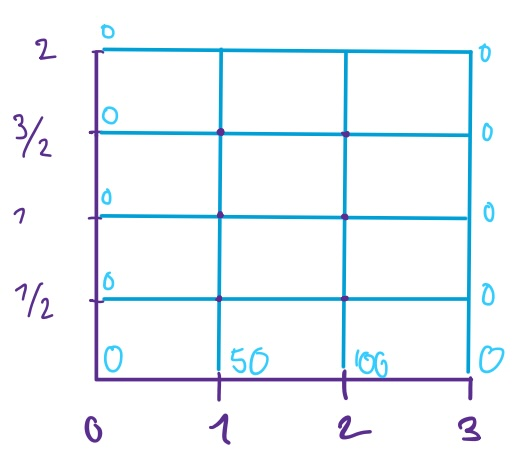
\includegraphics[width=0.4\columnwidth]{images/crank_nicolson}}

\textbf{Solution}

With $r = \frac{\Delta t}{\Delta x^2} = \frac{\sfrac{1}{2}}{1} = 0.5$, we receive the matrices
\begin{align*}
	F = \begin{bmatrix}
		3 & -0.5 \\
		-0.5 & 3
	\end{bmatrix},
	G = \begin{bmatrix}
		1 & 0.5 \\
		0.5 & 1
	\end{bmatrix}
\end{align*}

and thus
\begin{align*}
	\begin{bmatrix}
		\utild_1 \\
		\utild_2
	\end{bmatrix}^{(k+1)}
	=
	F^{-1} G
	\begin{bmatrix}
		\utild_1 \\
		\utild_2
	\end{bmatrix}^{(k)}
	\Rightarrow
	\begin{bmatrix}
		\utild_1 \\
		\utild_2
	\end{bmatrix}^{(4)}
	=
	(F^{-1} G)^4
	\begin{bmatrix}
		\utild_1 = 50 \\
		\utild_2 = 100
	\end{bmatrix}^{(0)}
\end{align*}







        \numericsubsection{Finite Elements}

We have a set of given local basis functions $v_1(x), \ldots, v_n(x)$ that are continuous and piecewise differentiable.
We subdivide $\Omega$ into meshes and assign each nodal point a nodal variable $a_k$.
Then, we use shape functions to represent the PDE on the mesh,
e.g. using triangular functions $l_1(x)=1-x$ and $l_2(x) = x$ to obtain \emph{local} element matrices
\begin{align*}
	E = 
	\begin{bmatrix}
		\int_0^1 l_1^\prime(s)\cdot l_1^\prime(s)\ ds & \int_0^1 l_1^\prime(s)\cdot l_2^\prime(s)\ ds \\
		\int_0^1 l_2^\prime(s)\cdot l_1^\prime(s)\ ds & \int_0^1 l_2^\prime(s)\cdot l_2^\prime(s)\ ds
	\end{bmatrix}
	=
	\begin{bmatrix}
		1 & -1 \\
		-1 & 1
	\end{bmatrix}
\end{align*}

that can then be used to construct the mesh matrix $M=1/h\cdot E$ using mesh size $h$.
Afterwards, the global Ritz matrix can be computed, e.g. for a one-dimensional mesh with 4 nodal points and 2 unknown inner points,
yielding 4 base functions $v_1,v_2,v_3,v_4$:

\begin{align*}
	R^4 = \begin{bmatrix}
		{\color{red} M^{(1)}_{0,0}} & \color{red}{M^{(1)}_{0,1}} & 0 & 0 \\
		{\color{red} M^{(1)}_{1,0}} & {\color{red} M^{(1)}_{1,1}} + {\color{blue} M^{(2)}_{0,0}} & {\color{blue} M^{(2)}_{0,1}} & 0 \\
		0 & {\color{blue} M^{(2)}_{1,0}} & {\color{blue} M^{(2)}_{1,1}} + {\color{green} M^{(3)}_{0,0}} & {\color{green} M^{(3)}_{0,1}} \\
		0 & 0 & {\color{green} M^{(3)}_{1,0}} & {\color{green} M^{(3)}_{1,1}}
	\end{bmatrix}
\end{align*}

The system vector can then be calculated:

\begin{align*}
	\vec{r^4} = \begin{pmatrix}
		\int_0^1 f(x)\cdot v_0(x)\ dx \\
		\vdots \\
		\int_0^1 f(x)\cdot v_3(x)\ dx
	\end{pmatrix}
\end{align*}

Finally, we have obtained the Ritz system: $R^4\cdot\vec{a}=\vec{r^4}$.
That yields the approximation function (as defined by the ansatz): $\tilde{u}(x)=\sum_{i=0}^3 a_i\cdot v_i(x)$
3with $a_0$ and $a_3$ fulfilling the boundary conditions.
        \newpage
        \section{Cheat Sheet}
\subsection{Roots}

\begin{align*}
	\sqrt[n]{a}\cdot\sqrt[n]{b} & = \sqrt[n]{a\cdot b} \\
	\frac{\sqrt[n]{a}}{\sqrt[n]{b}} & = \sqrt[n]{\frac{a}{b}} \\
	(\sqrt[n]{a})^m & = \sqrt[n]{a^m} \\
	\sqrt[m]{\sqrt[n]{a}} & = \sqrt[m\cdot n]{a}
\end{align*}


\subsection{Logarithm}

\begin{align*}
	\log_n(a\cdot b) & = \log_n(a) + \log_N(b) \\
	\log_n(a\div b) & = \log_n(a) - \log_N(b) \\
	\log_n(a^b) & = b \cdot \log_n(a)
\end{align*}

\subsection{Trigonometry}

\begin{align*}
	\tan\theta & = \frac{\sin\theta}{\cos\theta} \\
	\sin -\theta & = -\sin\theta\text{ (cos same)} \\
	\sin 2\theta & = 2\sin\theta\cos\theta \\
	\cos 2\theta & = 2\cos^2\theta - \sin^2\theta = 2\cos^2\theta - 1 = 1 - 2\sin^2\theta \\
	\sin(\alpha \pm \beta) & = \sin\alpha\cos\beta\pm\cos\alpha\sin\beta \\
	\cos(\alpha\pm\beta) & = \cos\alpha\cos\beta \mp \sin\alpha\sin\beta \\
	\sinh x & = \frac{e^x - e^{-x}}{2}=\frac{e^{2x}-1}{2e^x} \\
	\cosh x & = \frac{e^x + e^{-x}}{2} = \frac{e^{2x}+1}{2e^x} \\
	\tanh x & = \sinh x \div \cosh x \\
	\coth x & = \cosh x \div \sinh x \\
	\mathrm{sech}\ x & = 1 \div \cosh x = 2 \div (e^x+e^{-x})
\end{align*}

\subsection{Derivatives}
\begin{tabular}{r|l}
	$f(x)$ & $\frac{df}{dx}$ \\
	\hline
	$\sinh(x)$ & $\cosh(x)$ \\
	$\cosh(x)$ & $\sinh(x)$ \\
	$\mathrm{arcsinh}(x)$ & $1 \div \sqrt{x^2+1}$ \\
	$\mathrm{arccosh}(x)$ & $1 \div \sqrt{x^2 - 1}$ ($1<x$) \\
	$\tan(x)$ & $\cos^{-2}(x)$ \\
	$\log(x)$ & $x^{-1}$
\end{tabular}

\subsection{Integrals}
\begin{tabular}[h]{rl}
	$\int x^n\ dx$ & $= \frac{1}{n+1}x^{n+1} + C$ \\
	$\int \frac{1}{x}\ dx$ & $= \ln |x| + C$ \\
	$\int \frac{1}{ax + b}\ dx$ & = $\frac{1}{a} \ln |ax+b| + C$ \\
	$\int \frac{1}{(x+a)^2}\ dx$ & $= -\frac{1}{x+a} + C$ \\
	$\int \frac{1}{1 + x^2}$ & $= \tan^{-1} x + C$ \\
	$\int \ln ax\ dx$ & $= x\ln ax - x + C$ \\
	$\int e^{ax}\ dx$ & $= \frac{1}{a} e^{ax} + C$ \\
	$\int \sin(ax)\ dx$ & $= -\frac{1}{a}\cos(ax) + C$ \\
	$\int \sin^2(ax)\ dx$ & $= \frac{x}{2}-\frac{\sin(2ax)}{4a} + C$ \\
	$\int x\cos x\ dx$ & $= \cos x + x\sin x + C$ \\
	$\int \sinh(ax)\ dx$ & $= a^{-1}\cosh{ax} + C$ \\
	$\int \cosh(ax)\ dx$ & $= a^{-1}\sinh{ax} + C$ \\
\end{tabular}

\subsection{Integration Techniques}
\subsubsection{Integration by Parts}
\begin{equation*}
	\int_a^b u(x)v'(x)\ dx = \left[ u(x)v(x) \right]_a^b-\int_a^bu'(x)v(x)\ dx
\end{equation*}

Or, with $u=u(x)$, $du=u'(x)\ dx$, $v=v(x)$ and $dv=v'(x)\ dx$:
\begin{equation*}
	\int u\ dv=uv - \int v\ du
\end{equation*}

\subsubsection{Substitution}
\begin{equation*}
	\int_a^b f(g(x))\cdot g'(x)\ dx = \int_{g(a)}^{g(b)}f(u)\ du
\end{equation*}

\subsubsection{Leibniz Integral Rule}
\begin{multline*}
	\frac{d}{dx}\left(\int_{a(x)}^{b(x)}f(x,t)\ dt\right)
	=
	\\
	f(x,b(x))\cdot\frac{d}{dx}b(x)
	-f(x,a(x))\cdot\frac{d}{dx}a(x)
	+\int_{a(x)}^{b(x)}\frac{\partial}{\partial x}f(x,t)\ dt
\end{multline*}
Special case where $a(x)=a=\mathrm{const.}$ and $b(x)=b=\mathrm{const.}$:
\begin{equation*}
	\frac{d}{dx}\left(\int_a^b f(x,t)\ dt\right)
	=\int_a^b\frac{\partial}{\partial x}f(x,t)\ dt
\end{equation*}

\subsection{Particular Solutions to Simple ODEs}

\begin{tabular}[h]{rcl}
	$f'(x)=\frac{c}{x}f(x)$ & $\Rightarrow$ & $f(x)=k_1y^c$ \\
	$f'(x)=x\cdot f(x)$ & $\Rightarrow$ & $f(x)=k_1e^{cx}$ \\
	$f''(x) = c\cdot f(x)$ & $\Rightarrow$ & $f(x) = k_1e^{\sqrt{c}x}+k_2e^{-\sqrt{c}x}$ \\
	$f''(x) = -c\cdot f(x)$ & $\Rightarrow$ & $f(x)=k_1\sin(\sqrt{c}x)+k_2\cos(\sqrt{c}x)$ \\
	$f'(x)+af(x) = b$ & $\Rightarrow$ & $f(x) = \left(f(0)-\frac{b}{a}\right)e^{-ax}+\frac{b}{a}$
\end{tabular}

\subsection{Harmonic Function}

A function is harmonic if it fulfils $\Delta f = 0$. The mean value property applies:
\begin{align*}
	u(x) = \frac{1}{\mu(S_r(x))}\int_{S_r(x)}u(y)\ d\mu(y)
\end{align*}

\subsection{Polar Coordinates}
\begin{align*}
	x = r\cos \varphi \\
	y = r\sin \varphi
\end{align*}

The Laplace operator in polar coordinates is
\begin{align*}
	\Delta u = \frac{1}{r}\frac{\partial}{\partial r}
	\left(r\frac{\partial u}{\partial r}\right)
	+\frac{1}{r^2}\frac{\partial^2 u}{\partial \varphi^2}
\end{align*}
    \end{multicols}
\end{document}
